%\documentclass[a4paper,11pt]{article}%JHEP%
%\pdfoutput=1 % if your are submitting a pdflatex (i.e. if you have
             % images in pdf, png or jpg format)%JHEP%

%\usepackage{jheppub} % for details on the use of the package, please
                     % see the JHEP-author-manual%JHEP%

\documentclass[aps,prd,nofootinbib,preprint]{revtex4}

\usepackage[T1]{fontenc} % if needed
\usepackage{amsmath}
\usepackage{leftidx}
\usepackage{multirow}
\usepackage{enumerate}
%\usepackage{textcomp}

%\usepackage{underscore}
\usepackage[utf8]{inputenc}
\usepackage[english]{babel}

\usepackage[nottoc]{tocbibind}

\usepackage{hyperref}
%\usepackage{ulem}
\usepackage{color}
\usepackage{xcolor}
\usepackage{graphicx}
\usepackage{multirow}
\usepackage{amsmath,amssymb,amsthm,amsxtra,overpic,bbm,bm,float
,epsfig}



%JHEP%
%\title{\boldmath  Flavour Symmetry Embedded - GLoBES (FaSE-GLoBES)}


%JHEP%
%\author[a]{Jian Tang,}
%\author[a]{Tse-Chun Wang}
%\affiliation[a]{School of Physics, Sun Yat-Sen University, Guangzhou 510275, China}
%\emailAdd{tangjian5@mail.sysu.edu.cn}
%\emailAdd{wangzejun@mail.sysu.edu.cn}
%\abstract{Abstract...}


%\fontsize{3}{5}\selectfont
\begin{document} 
%\title{The user manual: FlAvour Symmetry with the GLoBES library}
%\title{FlAvour Symmetry with the GLoBES library}
\title{Flavour Symmetry Embedded - GLoBES (FaSE-GLoBES)} %JHEP%
%\maketitle %JHEP%
%\flushbottom %JHEP%
\author{Jian Tang$^1$\footnote{tangjian5@mail.sysu.edu.cn}}
\author{Tse-Chun Wang$^1$\footnote{wangzejun@mail.sysu.edu.cn}}
\affiliation{$^1$School of Physics, Sun Yat-Sen University, Guangzhou 510275, China}

\begin{abstract}
We present a supplemental tool \textbf{F}l\textbf{a}vour \textbf{S}ymmetry \textbf{E}mbedded (\textbf{FaSE}) for  \textbf{G}eneral \textbf{Lo}ng \textbf{B}aseline \textbf{E}xperiment \textbf{S}imulator (\textbf{GLoBES}). \textbf{FaSE}  works with \textbf{GLoBES} (\textbf{FaSE-GLoBES}) to analysis how flavour symmetry models can be examined with simulated neutrino oscillations. It can translate the model to oscillation parameters, and provides prior functions, in a user-friendly way. We demonstrate two examples for \textbf{FaSE-GLoBE}: how model parameters can be constrained and how a model can be excluded by an experiment. Finally, we emphasis as \textbf{GLoBES} is now a popular and power tool for neutrino oscillation physics, \textbf{FaSE} is convenient for flavour-symmetry model builders and neutrino oscillation phenomenologists.\\
\textbf{Keywords: Neutrino Oscillations, Leptonic Flavour Symmetry}  
\end{abstract} 

\maketitle

\section{Introduction}\label{sec:intro}

The discovery of neutrino oscillations points out the fact that neutrinos have mass, and provides evidence beyond the Standard Model (BSM). This phenomenon is successfully described by a theoretical framework with the help of three neutrino mixing angles ($\theta_{12}$, $\theta_{13}$, $\theta_{23}$), two mass-square splittings ($\Delta m_{21}^2$, $\Delta m_{31}^2$), and one Dirac CP phase ($\delta$) \cite{Pontecorvo:1967fh,Maki:1962mu,Pontecorvo:1957qd,Esteban:2018azc}. Thanks to the great efforts in the past two decades, we almost have a complete understanding of such a neutrino oscillation framework. More data in the neutrino oscillation experiments is needed to determine the sign of $\Delta m_{31}^2$, to measure the value of $\sin\theta_{23}$, to discover the potential CP violation in the leptonic sector and even to constrain the size of $\delta$ \cite{Esteban:2018azc}. For these purposes, the on-going long baseline experiments (LBLs), such as the NuMI Off-axis $\nu_e$ Appearance experiment (NO$\nu$A)~\cite{Ayres:2007tu} and the Tokai-to-Kamioka experiment (T2K)~\cite{Abe:2011ks}, can answer these questions with the statistical significance $\gtrsim 3\sigma$ in most of the parameter space. Based on the analysis with their data, the normal mass ordering ($\Delta m_{31}^2>0$), the higher $\theta_{23}$ octant ($\theta_{23}>45^\circ$), and $\delta\sim270^\circ$ are preferred so far~\cite{Esteban:2018azc}. The future LBLs, Deep Underground Neutrino Experiment (DUNE)~\cite{Acciarri:2015uup}, Tokai to Hyper-Kamiokande (T2HK)~\cite{Abe:2014oxa}, and the medium baseline reactor experiment, the Jiangmen Underground Neutrino Observatory (JUNO)~\cite{Djurcic:2015vqa,An:2015jdp} will further complete our knowledge of neutrino oscillations.

Flavour symmetry models are used to explain the origin of the neutrino mixing, and to predict the value of oscillation parameters (some of useful review articles are~\cite{Altarelli:2010gt,Ishimori:2010au,King:2013eh,King:2014nza,King:2015aea,King:2015ata,King:2017guk}). These models are motivated by some interesting features, \textit{such as} $\theta_{12}\sim 33^\circ$, and $\theta_{23}\sim 45^\circ$. Before the discovery of non-zero $\theta_{13}$ measurement by Daya Bay experiment~\cite{An:2013zwz}, the `tri-bi-maximal' neutrino mixing (TBM) ansatz, which was proposed in 2002 by Horrison, Perkins, and Scott~\cite{Harrison:2002er}, fitted with the experimental data in a good agreement:
\begin{equation*}
U_{\text{TBM}}=\left(
\begin{array}{ccc}
2/\sqrt{6} & 1/\sqrt{3} & 0\\
-1/\sqrt{6} & 1/\sqrt{3} & 1/\sqrt{2}\\
1/\sqrt{6}  & -1/\sqrt{3} & 1/\sqrt{2}
\end{array}\right).
\end{equation*} 
With the fact that $\theta_{13}\approx 8^\circ$, several ways to obtain such non-zero value of $\theta_{13}$ are proposed. One of popular proposals is to correct the tri-bi-maximal neutrino mixing such that 
\begin{equation*}
\sin\theta_{12}=(1+s)/\sqrt{3},~\sin\theta_{13}=r/\sqrt{2},~\text{and}~\sin\theta_{23}=(1+a)/\sqrt{2}.
\end{equation*}

Currently, some works discuss on how the future experiments can be used for testing these flavour symmetry models in the phenomenological point of view, \textit{e.g.}~Ref.~\cite{Ballett:2016yod,Chatterjee:2017xkb,Ding:2019zhn,Tang:2019edw}. A large number of these works are based on the \texttt{c}-library -- \textbf{G}eneral \textbf{Lo}ng \textbf{B}aseline \textbf{E}xperiment \textbf{S}imulator (\textbf{GLoBES}) \cite{Huber:2004ka,Huber:2007ji}, which is a convenient simulation tool to simulate neutrino oscillation experiments via the Abstract Experiment Definition Language (AEDL). Some AEDL files for experiments are also available on \textbf{GLoBES} website, while the working group of DUNE experiment also releases their AEDL files~\cite{Alion:2016uaj}.  \textbf{GLoBES} can be taken as one of popular and useful tools in the community of neutrino oscillation physics. However, it has not yet to be extended for the purpose of analysing flavour symmetry models.  In this work, we will present our simulation tool \textbf{F}l\textbf{a}vour \textbf{S}ymmetry \textbf{E}mbedded - \textbf{GLoBES} (\textbf{FaSE-GloBES}) that is a simulation code based on GLoBES library for studying the flavour symmetry. \textbf{FaSE} is a supplemental tool for GLoBES, written in \texttt{c/c++} language, and FASE-GLoBES allows the user to assign the flavour symmetry model and analysis how a flavour symmetry model can be excluded by the simulated neutrino oscillation experiment.




\section{Overview FASE-GloBES}

\textbf{F}l\textbf{a}vor \textbf{S}ymmetry \textbf{E}mbedded (\textbf{FaSE}) is a supplemental tool for \textbf{G}eneral \textbf{Lo}ng \textbf{B}aseline \textbf{E}xperiment \textbf{S}imulator (\textbf{GLoBES}) in order to analysis how a leptonic flavour symmetry model can be tested in neutrino oscillation experiments. \textbf{FaSE} is written in the \texttt{c/c++} language, and consist with three codes \textbf{FASE\_GLoBES.c} and \textbf{model-input.c}. The user defines the model in to \textbf{model-input.c}, while \textbf{FASE\_GLoBES.c} does not need to be touched. 

\begin{figure}[!h]%
\centering
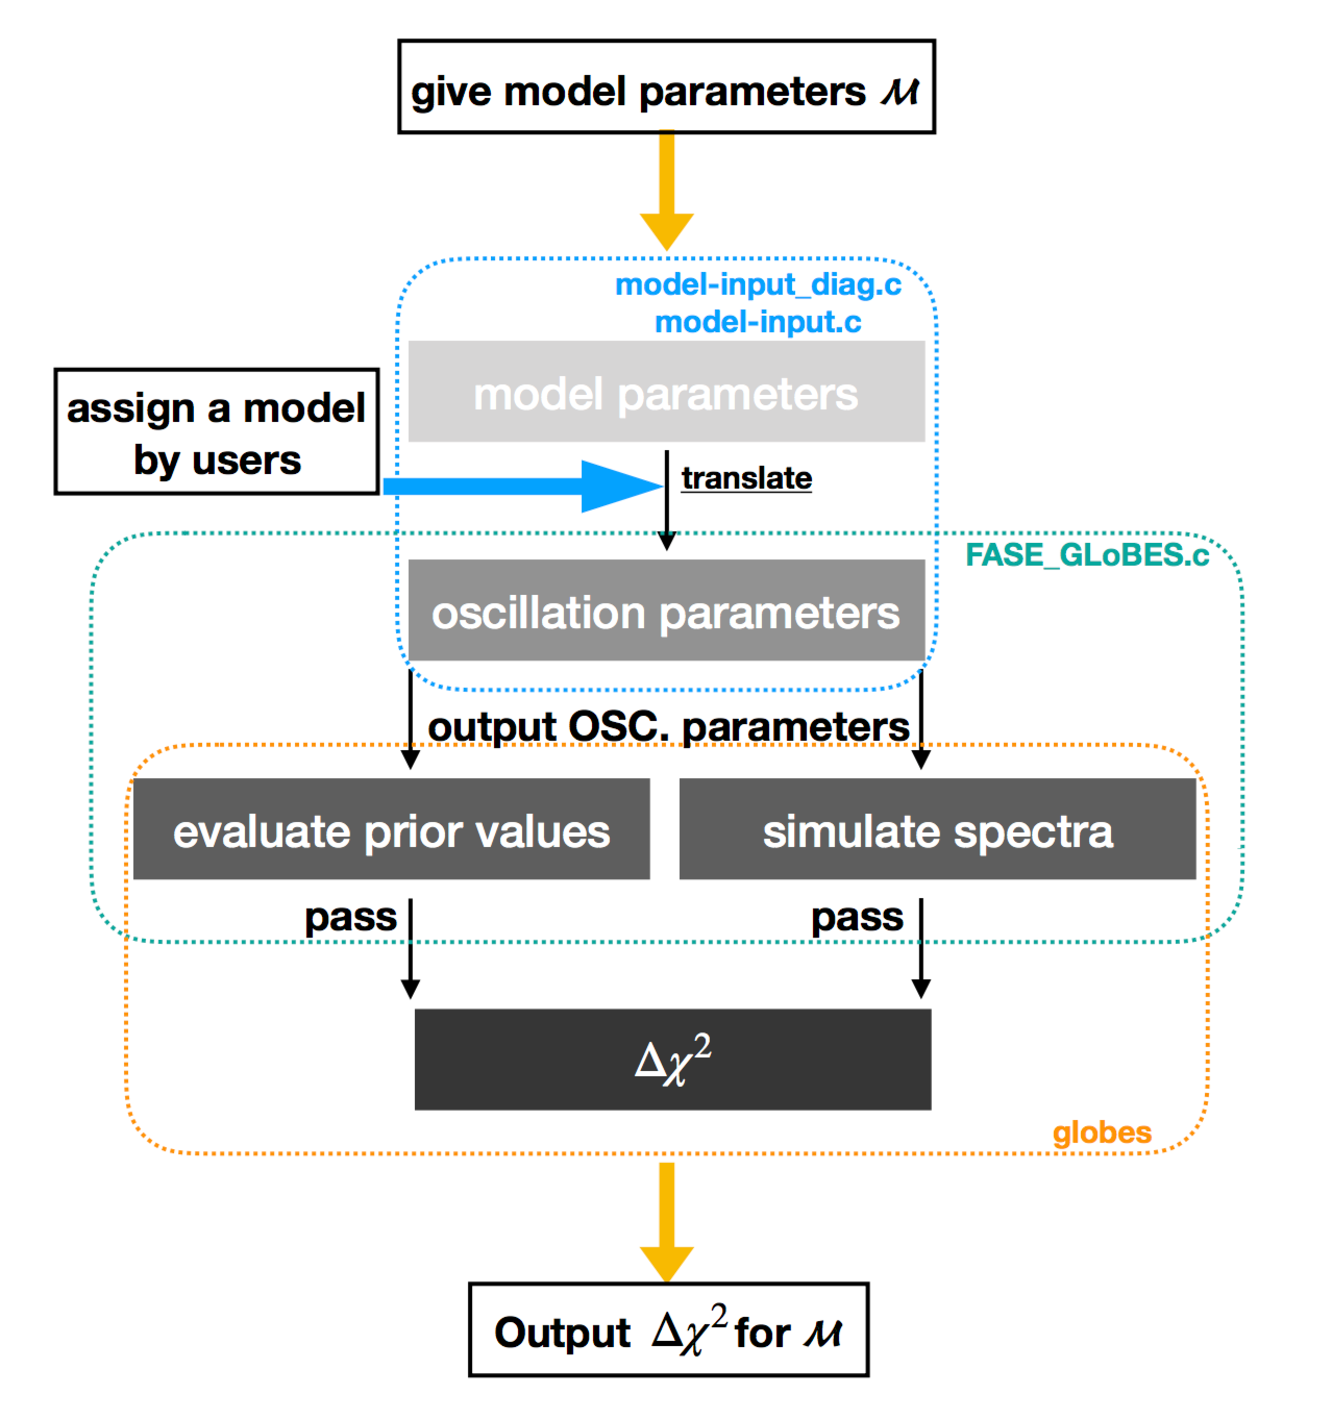
\includegraphics[width=4.5in]{Figs/FASE-chart_1_v1.pdf}
\caption{A scheme to correlate the model parameters with standard neutrino oscillation parameters. The error propagation is implemented in the simulation code up to the spectra analysis.}%
\label{fig:FASE}
\end{figure}


The concept of \textbf{FaSE-GLoBES} is shown in Fig.~\ref{fig:FASE}, in which three parts are shown: 1.~\textbf{the parameter translation} (the blue box), 2.~\textbf{giving oscillation-parameter values} (the green box), and 3.~\textbf{the $\chi^2$-value calculation} (the orange box). 
The idea behind this flow chart Fig.~\ref{fig:FASE} is that given a set of value for model parameter, the corresponding values for oscillation parameters are obtained by a translation, which is assigned by the user in \textbf{model-input.c}. And then, through \textbf{FASE\_GLoBES.c} these oscillation-parameter values are passed in to \textbf{GLoBES} library to simulate the event spectrum for evaluating the $\chi^2$ value. 


API functions in \textbf{FaSE} are listed:
\begin{enumerate}
\item \texttt{MODEL\_init($N_{para}$)},
\item  \texttt{FASE\_glb\_probability\_matrix},
\item  \texttt{FASE\_glb\_set\_oscillation\_parameters},
\item  \texttt{FASE\_glb\_get\_oscillation\_parameters},
\item \texttt{FASE\_prior\_OSC},
\item \texttt{FASE\_prior\_model}.
\end{enumerate}
The first one is to initialise \textbf{FaSE} with the number of input parameters $N_{para}$. The next three functions need to be included to replace the default \textbf{GLoBES} probability engine by the one that can read the output from \textbf{model-input.c}, as follows.\vspace{0.2cm}\\
\texttt{    glbRegisterProbabilityEngine(6,\\
                                 \&FASE\_glb\_probability\_matrix,\\
                                 \&FASE\_glb\_set\_oscillation\_parameters,\\
                                 \&FASE\_glb\_get\_oscillation\_parameters,\\
                                 NULL); }\vspace{0.2cm}\\ 
This probability engine can work with oscillation or model parameters. It can be set by the user with the parameter \texttt{PARA}. If \texttt{PARA=STAN} (\texttt{PARA=MODEL}) the probability engine works with oscillation (model) parameters. The final two items on the API list are prior functions. Once the user gives the prior in oscillation (model) parameters, the user needs to call \texttt{FASE\_prior\_OSC} (\texttt{FASE\_prior\_model}) as follows.\vspace{0.2cm}\\
\texttt{glbRegisterPriorFunction(FASE\_prior\_OSC,NULL,NULL,NULL); }  \\
or\\
\texttt{glbRegisterPriorFunction(FASE\_prior\_model,NULL,NULL,NULL); } \vspace{0.2cm}\\
We note that except for setting the probability engine and the prior function, the other parts in the main code should follow with the GLoBES manual. 


\section{Model setting}\label{sec:model_set}

The function \texttt{MtoS} can do the translator from model parameters $\vec{\theta}_{Model}$ to oscillation parameters $\vec{\theta}_{OSC.}$. After the user gives the array $\vec{\theta}_{Model}$ to the function \texttt{MtoS}, the output is the corresponding oscillation parameter $\vec{\theta}_{OSC.}$, of which components are $\theta_{12}$, $\theta_{13}$, $\theta_{23}$, $\delta$, $\Delta m_{21}^2$, and $\Delta m_{31}^2$. For the first four components, values are given in the unit of \textbf{rad}, while the other two are in \textbf{eV$^2$}. These values will be passed in to \textbf{FaSE\_GLoBES} to simulate 
the experimental spectra and compute the prior value.


To do the translation from $\vec{\theta}_{Model}$ to $\vec{\theta}_{OSC.}$, the user can assign the relation between the oscillation and model parameter sets, or define the mass matrix in model parameters, which will be diagonalised by the function \texttt{ModelTO} to obtain the corresponding oscillation-parameter values. 
%The relation between the oscillation and model parameter sets can be derived out by the user, 
In the way of directly giving the relation between oscillation and model parameter sets, the user needs to provide
\begin{equation}\label{eq:modelofOSC}
\vec{\theta}_{Model}=\vec{f}(\vec{\theta}_{OSC.})
\end{equation}
 in the function \texttt{MtoS}.
%

The oscillation parameters can also be obtained in the way based on
\begin{equation}\label{eq:MM}
U^\dagger\mathcal{M}\mathcal{M}^\dagger U = \mathbf{M}^2,~\text{where}~\mathbf{M}^2_{\alpha\beta}=m_\alpha^2\delta_{\alpha\beta},
\end{equation}
where $\mathcal{M}$ ($\mathbf{M}$) is the neutrino mass matrix in the flavour (mass) state. The matrix $\mathcal{M}$ is given by user with model parameters $\vec{\theta}_{Model}$. The matrix $U$ is the neutrino mixing matrix, and can be used for getting mixing angles. The difference between any two diagonal elements of $\textbf{M}$ ($\textbf{M}_{ii}-\textbf{M}_{jj}$) is the mass-squared difference ($\Delta m_{ij}^2$). This diagnolisation Eq.~\ref{eq:MM} can be done with the function \texttt{ModelTO}, which needs to be called in \texttt{MtoS} and outputs directly the vector $\vec{\theta}_{OSC.}$.


\section{Prior setting}\label{sec:prior}
Given a set of values for model parameters, \textbf{FASE\_GLoBES.c} will obtain the corresponding oscillation-parameter values from \textbf{model-input.c}, and will pass these values to simulate event spectra and to compute the prior value. Two gaussian prior functions are provided in \textbf{FaSE} -- \texttt{FASE\_prior\_OSC} and \texttt{FASE\_prior\_model}. These two functions are for different purposes. If the user give the prior in oscillation (model) parameters, the user should register \texttt{FASE\_prior\_OSC} (\texttt{FASE\_prior\_model}) with the \textbf{GLoBES} function \texttt{glbRegisterPriorFunction}, as we introduced in the beginning of this section. The user also needs to assign the parameter \texttt{PARA=STAN} (\texttt{PARA=Model}), when the user prefers to give the prior in oscillation (model) parameters. The Gaussian prior is 
\begin{equation}\label{eq:prior}
\chi^2_{prior}=\sum_{i} \frac{(\theta_i-\theta^c_i)^2}{\sigma_i^2},
\end{equation}
 where $\theta_i$ is one of parameters constrained by prior, $\theta^c_i$ ($\sigma_i$) is the central value (Gaussian width) of the prior for $\theta_i$. We note that $\theta_i$ can be either model ($\vec{\theta}_{Model}$) or oscillation parameters ($\vec{\theta}_{OSC.}$).
%
The values of $\theta^c_i$ and $\sigma_i$ need to be given by the user through three arrays: \texttt{Central\_prior}, \texttt{UPPER\_prior}, and \texttt{LOWER\_prior}, in which there are six components. To treat asymmetry of width for upper ($\theta_i>\theta_i^c$) and lower ($\theta_i<\theta_i^c$) Gaussian widths, we give values in two arrays \texttt{UPPER\_prior}, and \texttt{LOWER\_prior}, respectively. If the user gives the prior in model parameters, the order of each component follows with the setup of input of the probability engine. While the user gives the prior in oscillation parameters, the six components in order are $\theta_{12}$, $\theta_{13}$, $\theta_{23}$, $\delta$, $\Delta m_{21}^2$, and  $\Delta m_{31}^2$. The first four parameter are in \textbf{rad}, and the final two are in \textbf{eV$^2$}.

Finally, some restrictions are imposed by the studied flavour symmetry model. We set up these restrictions in the function \texttt{model\_restriction} in \texttt{model-input.c}. In the function \texttt{model\_restriction}, the user needs to \textit{return $1$} once the restriction is broken. For example, if the normal ordering is imposed, we give ``\texttt{ if (DMS31<0) \{ return 1;\} } '' in \texttt{model\_restriction}, where \texttt{DMS31} is the variable for $\Delta m_{31}^2$. Then, when the restriction is broken, \texttt{model\_restriction} returns the value $1$ to the prior function \texttt{FASE\_prior\_OSC} or \texttt{FASE\_prior\_model}. 
%In the following, the prior function will give $10^6$ for the $\chi^2$ value, and it will be selected out when the user studies the statistically reasonable region in the parameter space.  

\section{The definition for $\chi^2$ (based on \textbf{GLoBES})}\label{sec:chi-squared}
% {\color{red}CAN BE REMOVED}
 
The user can use \textbf{FaSE-GLoBES} to study the constraint of model parameters. The expression of $\chi^2$ is used as the default \textbf{GLoBES} setting. In more detail, the $\chi^2$ function is constructed based on a log-likelihood ratio,
\begin{equation}\label{eq:chi-squared}
\chi^2(\vec{\theta}^{hyp.},\xi_s,\xi_b)=2\sum_i\left(\eta_i(\vec{\theta}^{hyp.},\xi_s,\xi_b)-n_i+n_i\ln\frac{n_i}{\eta_i(\vec{\theta}^{hyp.},\xi_s,\xi_b)} \right)+p(\xi_s,\sigma_s)+p(\xi_b,\sigma_b)+\chi^2_{prior},
\end{equation}
where $i$ runs over the number of bins, $\eta_i(\vec{\theta},\xi_s,\xi_b)$ is the hypothesis event rate for bin i and $E_i$ is the central bin energy. The vector $\vec{\theta}$ consists of test model or oscillation parameters. The parameters $\xi_s$ and $\xi_b$ are introduced to account for the systematic uncertainty of normalisation for the signal (subscript $_s$) and background (subscript $_b$) components for the event rate, and are allowed to vary in the fit as nuisance parameters. For a given hypothesised set of parameters $\vec{\theta}$, the event rate for bin $i$ is calculated as\\
\begin{equation}
\eta_i(\vec{\theta}^{hyp.},\xi_s,\xi_b)=(1+\xi_s)\times s_i+(1+\xi_b)\times b_i,
\end{equation}
where $s_i$ and $b_i$ are the expected number of signal and background events in bin $i$, respectively. The nuisance parameters are constrained by the Gaussian prior $p(\xi,\sigma)=\xi^2/\sigma^2$ with corresponding uncertainties $\sigma_s$ and $\sigma_b$ for the signal and background, respectively. Finally, $\chi^2_{prior}$ is a set of Gaussian priors for hypothesis, and is expressed as Eq.~\ref{eq:prior}. After doing all minimisations, the user obtain the $\chi^2$ value for a specific hypothesis $\vec{\theta}^{hyp.}$, $\chi^2(\vec{\theta}^{hyp.})$.


Based on the $\chi^2$ value Eq.~\ref{eq:chi-squared}, we can study how model parameters can be constrained and how a flavour-symmetry model can be tested by simulated experiments. In the following we will introduce how it works.

\subsection*{Applications}

The user of \textbf{FaSE-GLoBES} is able to study how model parameters can be constrained by the simulated experiment. To do so, the user needs to define the true event spectrum $n_i$ with a set of model ($\vec{\theta}_{Model}^{true}$) or oscillation parameters ($\vec{\theta}_{OSC.}^{true}$), \textit{i.e.}~set up $n_i(\vec{\theta}_{Model}^{true})$ or $n_i(\vec{\theta}_{OSC.}^{true})$. The hypothesis $\vec{\theta}_{Model}^{hyp.}$ predicts the tested event spectrum $\eta_i(\vec{\theta}_{Model}^{hyp.},\xi_s,\xi_b)$. With the default setting for $\chi^2$ function Eq.~\ref{eq:prior}, from \textbf{FaSE-GLoBES} the user computes the statistical quantity,
\begin{equation}\label{eq:chi_model}
\chi^2(\vec{\theta}_{Model}^{hyp.}),~~\text{with}~n_i(\vec{\theta}_{Model}^{true})~\text{or}~n_i(\vec{\theta}_{OSC.}^{true}).
\end{equation}
%
We note that the minimum of $\chi^2$ in the whole parameter space ($\chi^2_{min.}$) may not be $0$. Therefore, to study the precision of model parameters, the user should use the value $\Delta\chi^2(\vec{\theta}_{Model}^{hyp.})\equiv \chi^2(\vec{\theta}_{Model}^{hyp.})-\chi^2_{min.}$, instead of $\chi^2$ itself. By varying different hypothesis $\vec{\theta}_{Model}^{hyp.}$, the user can obtain the allowed region of model parameters with the statistical quantity $\Delta\chi^2(\vec{\theta}_{Model}^{hyp.})$. 

The user can also study how well a flavour symmetry model explains the computed data as predicting how the simulated experiment can exclude this model. In the other word, the user studies the minimum of $\chi^2$ for the flavour symmetry model $\vec{\theta}_{Model}$ as a hypothesis, assuming different true oscillation values, \textit{i.e.}~different $\vec{\theta}^{true}_{OSC}$. To do so, we compute the same statistical quantity Eq.~\ref{eq:chi_model}, while the true spectrum is varied with different true values $\vec{\theta}_{OSC}^{true}$. All model parameters are allowed to be varied with the user-defined prior.
%
Finally, the user needs to adopt Wilk's theorem \cite{Wilks:1938dza}. When comparing nested models, the $\Delta \chi^2$ test statistics is a random variable asymptotically distributed according to the $\chi^2$-distribution with the number of degrees of freedom, which is equal to the difference in the number of free model parameters \texttt{dof}. 

\section{Constraint of model parameters}

\textbf{FaSE-GloBES} can be used to study how the model parameter is constrained by simulated neutrino oscillation experiments. We take the tri-direct littlest seesaw (TDLS) model as example. Under this model, the light left-handed Majorana neutrino mass matrix is given by
\begin{equation}
\label{eq:mnu}  m_{\nu}=m_{a}\begin{pmatrix}
 1 &~ \omega  &~ \omega ^2 \\
 \omega  &~ \omega ^2 &~ 1 \\
 \omega ^2 &~ 1 &~ \omega  \\
\end{pmatrix}+e^{i\eta}m_{s}
\begin{pmatrix}
 1 &~  x &~  x \\
 x &~ x^2 &~ x^2 \\
 x &~ x^2 &~ x^2 \\
\end{pmatrix}\,,
\end{equation}
where $x$, $\eta$, $m_a$, and the ratio $r\equiv m_s/m_a$ are four parameters and will be constrained by experimental data. We note that from Eq.~(\ref{eq:mnu}), $m_1=0$ and the normal mass ordering are imposed, and will need to be imposed in \textbf{FaSE-GLoBES}. Therefore, the restrictions in this model are $m_a>0$ and $r>0$.
%\begin{figure}[!h]
% \flushleft
%\hspace{15mm}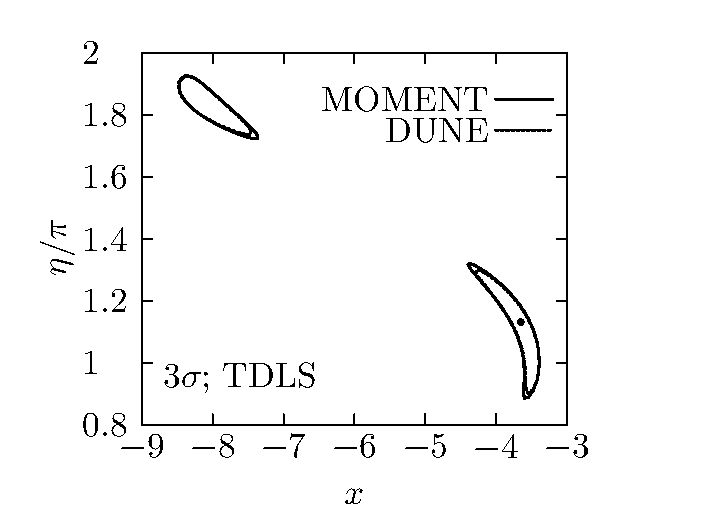
\includegraphics[width=0.32\textwidth]{figs/x_eta.pdf}$~~~~~~$\\
%\hspace{15mm} 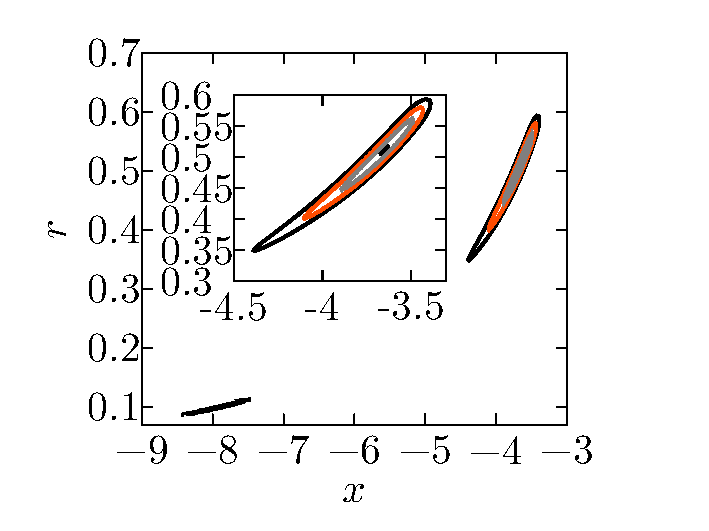
\includegraphics[width=0.32\textwidth]{figs/x_r.pdf}\hspace{-11mm}
% 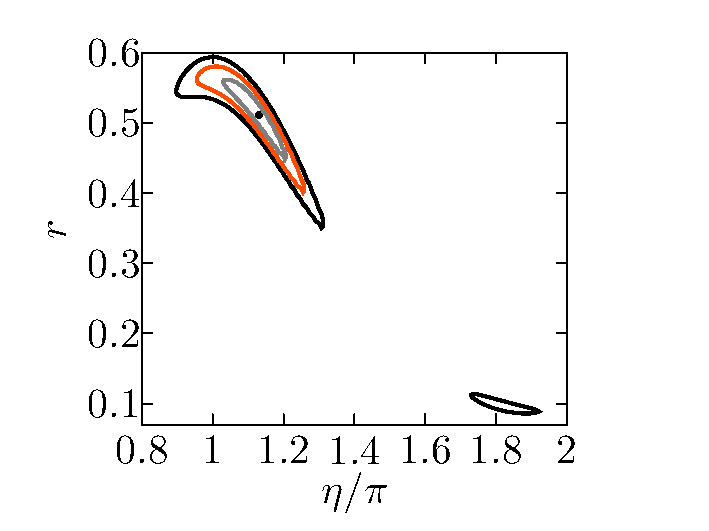
\includegraphics[width=0.32\textwidth]{figs/eta_r.pdf}$~~~~~~$\\
%\hspace{15mm} 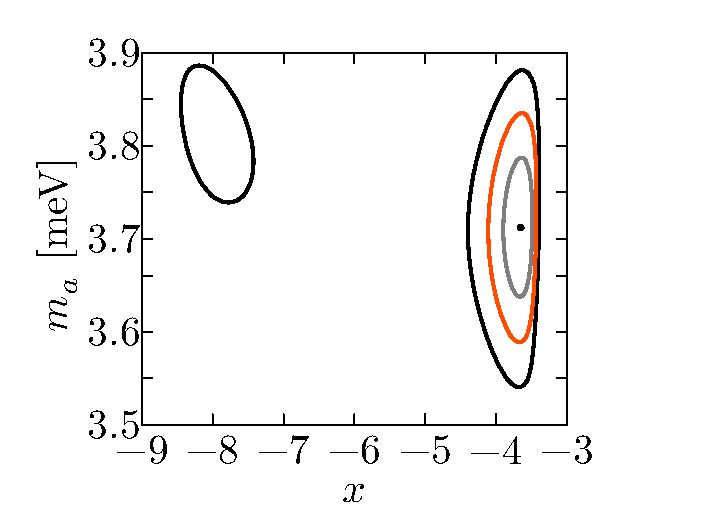
\includegraphics[width=0.32\textwidth]{figs/x_ma.pdf}\hspace{-11mm}
% 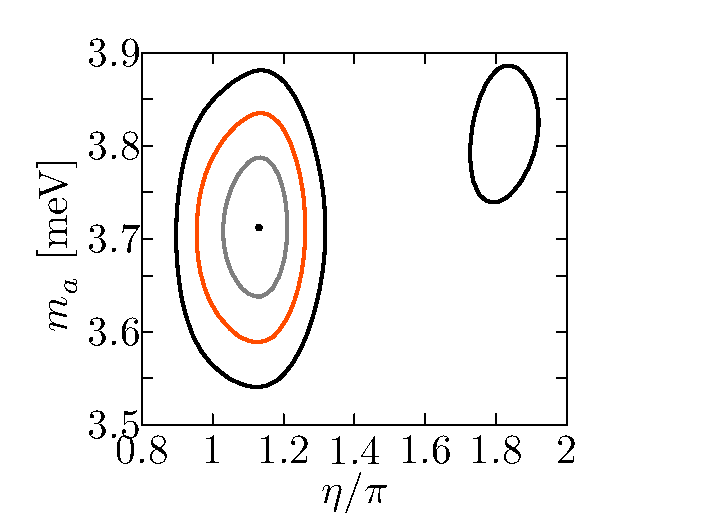
\includegraphics[width=0.32\textwidth]{figs/eta_ma.pdf}\hspace{-11mm}
% 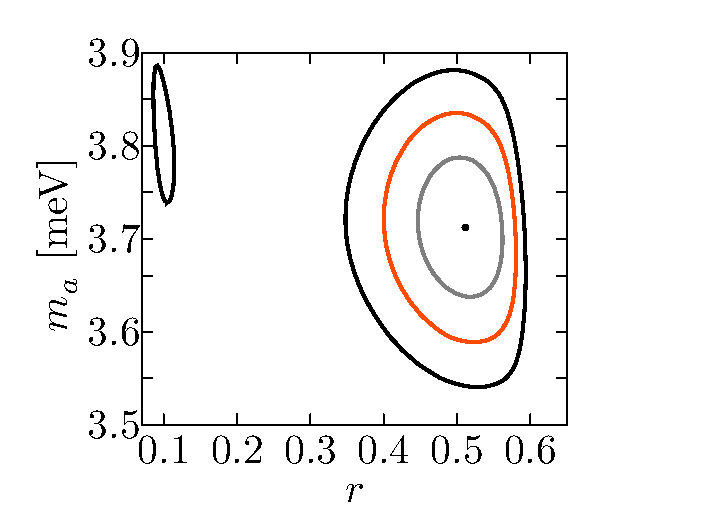
\includegraphics[width=0.32\textwidth]{figs/r_ma.pdf}
% \caption{\label{fig:model_2D}Precision measurements of any two model parameters at 3$\sigma$ confidence level in the framework of three neutrino oscillations taking uncertainties of the current global fit results, for MOMENT, at $1\sigma$ (gray), $2\sigma$ (orange), $3\sigma$ (black). True values for the model parameters are used $(x,~\eta,~r,~M_a)=(-3.65,~1.13\pi,~0.511,~3.71~\text{meV})$.}
%\end{figure}

\begin{figure}[!h]
 %\flushleft
 \centering
\hspace{15mm}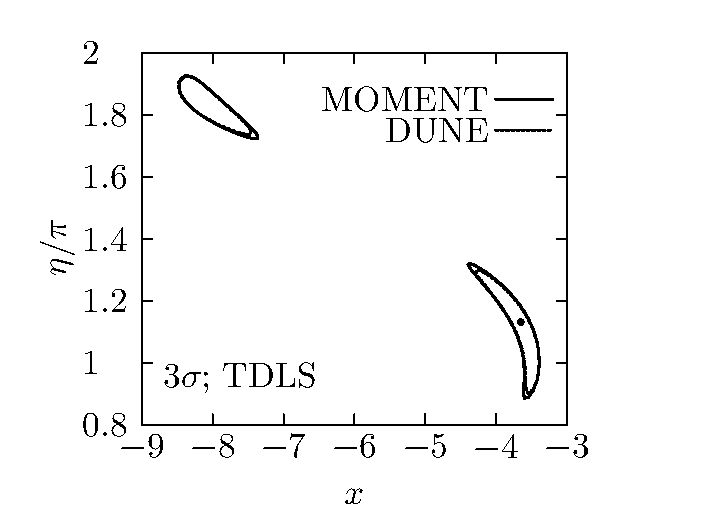
\includegraphics[width=0.5\textwidth]{figs/x_eta.pdf}
 \caption{\label{fig:x_eta}Precision measurements of any two model parameters in the framework of three neutrino oscillations taking uncertainties of the current global fit results, for MOMENT, at $1\sigma$ (gray), $2\sigma$ (orange), $3\sigma$ (black). True values for the model parameters are used $(x,~\eta,~r,~M_a)=(-3.65,~1.13\pi,~0.511,~3.71~\text{meV})$.}
\end{figure}

In Fig.~\ref{fig:x_eta}, we study how parameters $x$ and $\eta$ can be constrained by the MuOn-decay MEdium baseline NeuTrino beam experiment (MOMENT). We input the model by giving model parameters as functions of oscillation parameters Eq.~\ref{eq:modelofOSC}. And, parameters $r$ and $ma$ are varied with the prior that is given in oscillation parameters, according to the global-fit result NUFIT4.0. More details are presented in the user manual. The code for this example is provided as \textbf{x\_eta.c} in the \textbf{FaSE} distribution.


\section{Model testing}

\begin{figure}[!h]
 \centering
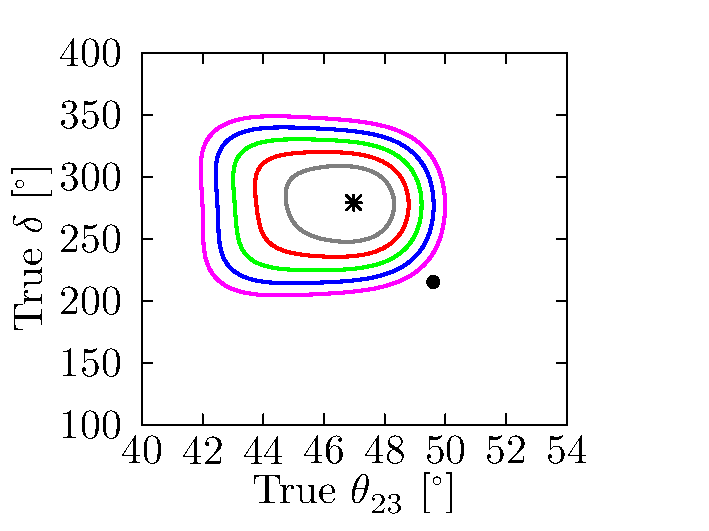
\includegraphics[width=0.5\textwidth]{figs/SR_th23_dCP.pdf}
\caption{\label{fig:th23_delta}The 2-D exclusion contour for tri-direct littlest seesaw model on the plane of two true standard parameters $\theta_{23}$ and $\delta$, from $1\sigma$ to $5\sigma$. The range for each parameter is taken according to the $3\sigma$ uncertainty in NuFit4.0 results. The black dot denotes the best fit of NuFit4.0 results ($(\theta_{12},~\theta_{13},~\theta_{23},~\delta,~\Delta m_{21}^2,~\Delta m_{31}^2)=(33.82^\circ,~8.61^\circ,~49.6^\circ,~215^\circ,~7.39\times10^{-5}~\text{eV}^2,~2.525\times10^{-3}~\text{eV}^2)$), while the star is the prediction by the tri-direct littlest seesaw model with NuFit4.0 results ($(\theta_{12},~\theta_{13},~\theta_{23},~\delta,~\Delta m_{21}^2,~\Delta m_{31}^2)\sim(36.25^\circ,~8.63^\circ,~47^\circ,~279^\circ,~7.39\times10^{-5}~\text{eV}^2,~2.525\times10^{-3}~\text{eV}^2)$).}
\end{figure}

We can also study on excluding the model, assuming different true values for oscillation parameters. In this example, we present testing the TDLS model in various true values of $\theta_{23}$ and $\delta$. We compute the minimal $\chi^2$ value for the tested model with all four model parameters, varied with the prior Eq.~\ref{eq:prior} according to NUFIT4.0 result. And, the studied statistics function is exactly Eq.~\ref{eq:chi-squared}, but the true event rate $n_i$ is predicted by a set of oscillation parameters, which will be varied in the code. 

Mentioned in Sec.~\ref{sec:chi-squared}, the user need to consider Wilk's theory with the different of degrees of freedom between the true theory and the hypothesis, \texttt{dof}. Here the number \texttt{dof} is $2$. And that is our output: \texttt{gsl\_cdf\_chisq\_Qinv(gsl\_cdf\_chisq\_Q(fabs(res),dof),1)}. We show the result in Fig.~\ref{fig:th23_delta}. More details are presented in the user manual. The code for this example is provided as \textbf{th23\_delta.c} in the \textbf{FaSE} distribution.



%\begin{figure}[!h]
 %\flushleft
%
%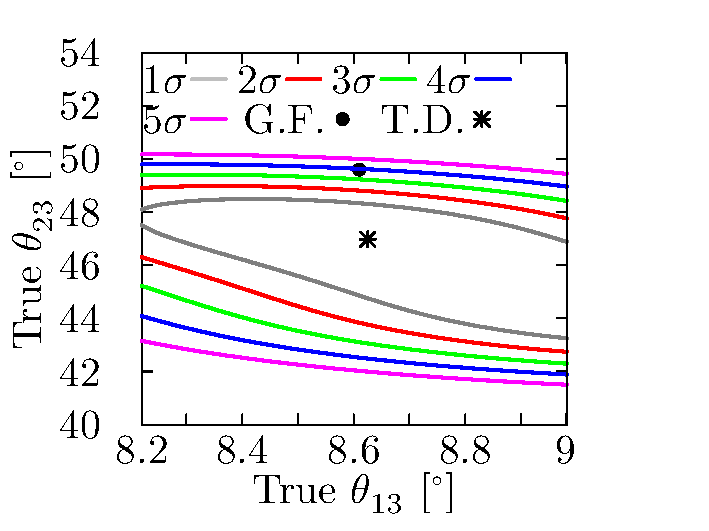
\includegraphics[width=0.32\textwidth]{figs/SR_th13_th23.pdf}$~~~~~~$\\
%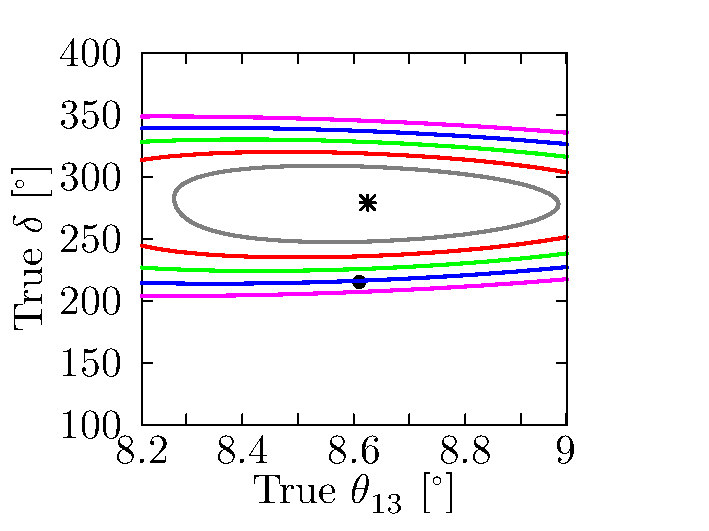
\includegraphics[width=0.32\textwidth]{figs/SR_th13_dCP.pdf}
%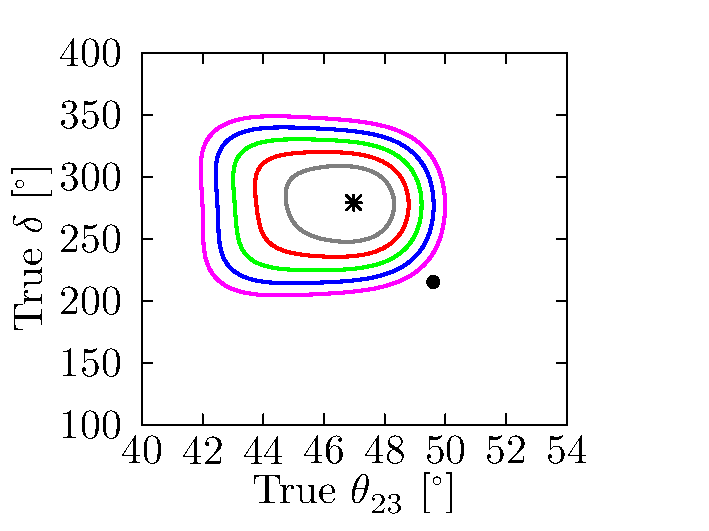
\includegraphics[width=0.32\textwidth]{figs/SR_th23_dCP.pdf}$~~~~~~$\\
%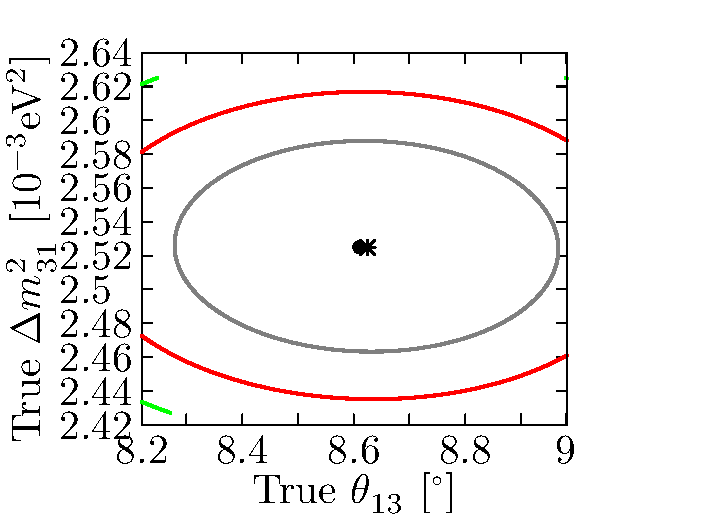
\includegraphics[width=0.32\textwidth]{figs/SR_th13_ldm.pdf}
%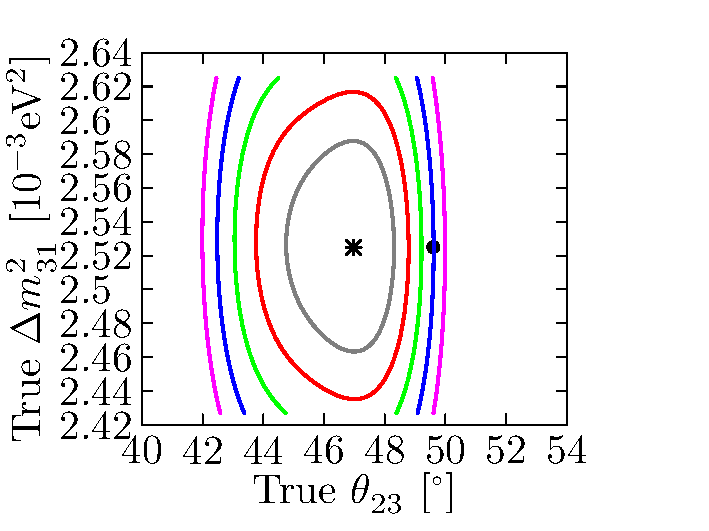
\includegraphics[width=0.32\textwidth]{figs/SR_th23_ldm.pdf}
%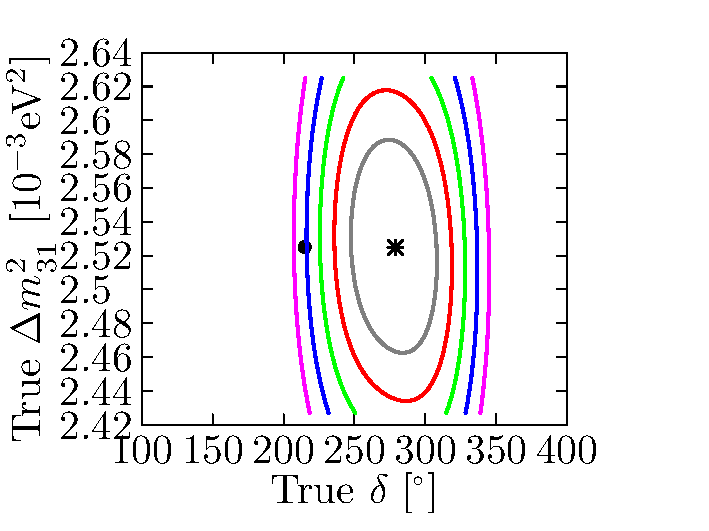
\includegraphics[width=0.32\textwidth]{figs/SR_dCP_ldm.pdf}
 %\caption{\label{fig:SR_2D}The 2-D exclusion contour for tri-direct littlest seesaw model on the plane of any two true standard parameters, from $1\sigma$ to $5\sigma$. The range for each parameter is taken according to the $3\sigma$ uncertainty in NuFit4.0 results. The black dot denotes the best fit of NuFit4.0 results ($(\theta_{12},~\theta_{13},~\theta_{23},~\delta,~\Delta m_{21}^2,~\Delta m_{31}^2)=(33.82^\circ,~8.61^\circ,~49.6^\circ,~215^\circ,~7.39\times10^{-5}~\text{eV}^2,~2.525\times10^{-3}~\text{eV}^2)$), while the star is the prediction by the tri-direct littlest seesaw model with NuFit4.0 results ($(\theta_{12},~\theta_{13},~\theta_{23},~\delta,~\Delta m_{21}^2,~\Delta m_{31}^2)\sim(36.25^\circ,~8.63^\circ,~47^\circ,~279^\circ,~7.39\times10^{-5}~\text{eV}^2,~2.525\times10^{-3}~\text{eV}^2)$).}
%\end{figure}


\section{Summary and conclusions}

We have presented \textbf{FaSE}, which is a supplemental simulation tool for \textbf{GLoBES} to study the flavour symmetry with neutrino oscillation experiments. \textbf{FaSE} provides \texttt{c}-codes: \textbf{model-input.c} and \textbf{FASE\_GLoBES.c}. Shown in Fig.~\ref{fig:FASE}, \textbf{FASE\_GLoBES}, which calls functions in \textbf{model-input.c}, plays a role as a bridge between \textbf{FaSE} and \textbf{GLoBES} to simulate the expected spectra and compute the prior value. It can be left to be untouched by users. However, all inputs of the user needs to be given in the code \textbf{model-input.c}. Given a set of model parameters $\vec{\theta}_{Model}$, with \textbf{GLoBES}, the output can be the $\chi^2$ value for the hypothesis $\vec{\theta}_{Model}$. 
%{\color{red}\texttt{Makefile} is easy to include these two binary files (\textbf{model-input} and \textbf{FASE\_GLoBES}) in the \texttt{makefile} script for \textbf{GLoBES}. }

We also present two examples for \textbf{FaSE-GLoBES} with the flavour symmetry model -- tri-direct littlest seesaw (TDLS) -- and the future neutrino oscillaiton experiment -- MOMENT. We show the model can be assign in two ways: the relation between model and oscillation parameters or the form of mass matrix in model parameters. The input of the oscillation probability and prior value can be in model or oscillation parameters. We further demonstrate how to use \textbf{FaSE-GLoBES} to obtain the constraint of any two of model parameters, and to study the ability to TDLS by MOMENT experiment. 

Finally, \textbf{GLoBES} is a popular and powerful simulation tool to analysis the neutrino oscillation experiments in a simple language (AEDL), without losing too much detail. Considering the success of the flavour symmetry theory to explain the neutrino oscillations, \textbf{FaSE-GLoBES} should benefit model builders of leptonic flavour symmetry and phenomenologists for neutrino oscillation physics. We leave the flexibility for the user, and some other improvements and extensions can be also expected in the future.
 
 \begin{acknowledgements}
\end{acknowledgements}

% BIBLIOGRAPHY
% use BIBTEX if you want
\bibliographystyle{JHEP}
%\bibliographystyle{plain}
\bibliography{FAS-GLoBES.bib}
\end{document}
